% LaTeX template for a short report (written for MSES scenario modelling)
% uses LaTeX documentclass "article" for use of sections (not chapter) and References (not Bibliography)
% for Chapters and Bibliography use "documentclass "report
\documentclass[10pt]{article}   % Use article class with 10pt letter
%\documentclass[10pt]{report}
\usepackage[utf8]{inputenc}

%\usepackage[T1]{fontenc}  % 8-bit encoding, helps hyphenation of accented characters -
% https://tex.stackexchange.com/a/677/42066

% Use A4 paper and set margins:
%\usepackage[a4paper, twoside, top=2.0cm, left=3.0cm, bottom=2.0cm, right=2.0cm]{geometry}
\usepackage[a4paper, twoside, top=2.0cm, left=2.0cm, bottom=2.0cm, right=2.0cm]{geometry}
%\usepackage[a4paper, top=2.5cm, left=2.5cm, bottom=2.5cm, right=2.5cm]{geometry}

\usepackage[english]{babel}  % Hyphenation and more for English

\usepackage{pgf}      % Include graphics inside figures using \pgfimage
\usepackage[font=small, labelfont=bf]{caption}  % Stylize figure, table, etc. captions

\usepackage{parskip}         % Replace paragraph indentations with white lines
\usepackage[hyphens]{url}    % Take care of urls, e.g. wrapping in the Bibliography (hyphens: also break at -)

\usepackage{xspace}   % \xspace saves the user from having to type \  or {} after a macro name in text.

% Use the appendix package for nicer appendices:
%\usepackage[toc,page]{appendix}  % MvdS
\usepackage[titletoc]{appendix}
%\usepackage[toc,page,title]{appendix}  % Use \begin{appendices} ... \end{} iso \appendix

% \usepackage[numbib,numindex]{tocbibind}  % Add ToC, List of Figures/Tables/Code listings, Bibliography and Index to ToC
% \usepackage[]{tocbibind}       % Add ToC, List of Figures/Tables/Code listings, Bibliography and Index to ToC
\usepackage[nottoc]{tocbibind}   % ToC without extra "Contents" entry...

\usepackage{amsmath,amssymb,bbm}
\usepackage{enumerate}         % Choose alternative numberings, e.g. \begin{enumerate}[a.]

\usepackage{listings}          % Code listings
\usepackage[section, above, below]{placeins}  % \FloatBarrier - flush floats before \section by default
% \usepackage{pgf}               % Figures

\usepackage{color}
\definecolor{lightgrey}{rgb}{0.9,0.9,0.9}
\definecolor{darkgreen}{rgb}{0.0,0.6,0.0}

% Citations:

% option1: use natbib/bibtex with MvdS_number_url.bst
%\usepackage[numbers, square]{natbib}  % Use numbered citations with square brackets
%\bibliographystyle{MvdS_number_url}  % Use [1], print url = field  (plain doesn't print urls)

%option2: use biblatex/biber without *.bst file
\usepackage[backend=biber, style=numeric, citestyle=numeric-comp, sorting=none]{biblatex} 
\setlength\bibitemsep{0.5\baselineskip}
\usepackage{csquotes}

% \bibliography{mybibliography} % old-style for backward comp. in preamble for biblatex/bibtex
\addbibresource{mybibliography.bib}  % new syntax for BibLaTeX


\usepackage{fancybox}  % Use \ovalbox for key strokes

\newcommand{\ldf}{\usefont{OT1}{cmr}{m}{n}}     % Select default LaTeX font - Computer Modern Roman
%\newcommand{\ldf}{\usefont{OT1}{cmss}{m}{n}}     % Select default LaTeX font - Computer Modern Sans
%\newcommand{\ldf}{\usefont{OT1}{phv}{m}{n}}     % Select default LaTeX font - Helvetica
\newcommand{\ttbf}{\usefont{OT1}{lmtt}{bx}{n}}  % Select bold typewriter font

%\usepackage[font=sf]{caption}  % Use sans-serif font for float captions - not exactly Helvetica



\newcommand{\note}[1]{\color{red}\textbf{#1}\color{black}\xspace}
\newcommand{\marc}[1]{\color{red}\textbf{Marc: #1}\color{black}\xspace}

\newcommand{\myChapter}[1]{
  \chapter{#1}
  \minitoc  % Create a ToC of this chapter
}


% General expressions:
\newcommand{\eg}{\emph{e.g.}\xspace}
\newcommand{\ie}{\emph{i.e.}\xspace}
\newcommand{\etc}{\emph{et cetera}\xspace}
\newcommand{\ff}{\emph{ff}\xspace}

% CLI symbols:
\newcommand{\pipe}{$|$}      % Needed to avoid | in \index{}
\newcommand{\logor}{$|\,|$}  % Needed to avoid | in \index{}
\newcommand{\home}{\url{~}}  % Home directory


% Often used code names:
\newcommand{\NULL}{\code{NULL}}
\newcommand{\void}{\code{void}}
\newcommand{\stdout}{\code{stdout}}
\newcommand{\stderr}{\code{stderr}}

% Man pages:
\newcommand{\man}[2]{\texttt{man #1 #2}\xspace}
\newcommand{\mancmd}[1]{\texttt{man #1}\xspace}

% Code:
\newcommand{\prototype}[3]{\hspace*{2em}\texttt{#1} {\ttbf #2\ldf}(\texttt{#3});\xspace}  % function prototype
\newcommand{\var}[2]{\hspace*{2em}\texttt{#1} {\ttbf #2\ldf};\xspace}  % variable declaration
\newcommand{\code}[1]{\texttt{#1}\xspace}  % inline code
\newcommand{\codeb}[1]{\ttbf #1\ldf\xspace}  % inline bold code
\newcommand{\codeline}[1]{\hspace*{2em}\texttt{#1}}  % separate code line

\newcommand{\cli}[1]{\noindent\hspace*{2em}\code{\$ #1}}  % command line input
\newcommand{\clir}[1]{\noindent\hspace*{2em}\code{\# #1}}  % command line input root
\newcommand{\clo}[1]{\noindent\hspace*{2em}\code{#1}}  % command line output
\newcommand{\clitem}[1]{\item[\code{\$}] \code{#1}}  % cli in itemized list, with $ as bullet
\newcommand{\clitemb}[1]{\item[\codeb{\$}] \codeb{#1}}  % cli in itemized list, with $ as bullet - bold

\newcommand{\key}[1]{\Ovalbox{\texttt{#1}}\xspace}  % key press/combination
\newcommand{\keyb}[1]{\Ovalbox{\ttbf #1\ldf}\xspace}  % key press/combination bold


% Heat pumps
\newcommand{\COP}{\mathrm{COP}}  % COP in "math mode"
\newcommand{\COPh}{\COP_{\mathrm{heating}}}  % COP_heating in "math mode"

\newcommand{\Qh}{Q_{\mathrm{H}}}
\newcommand{\Qc}{Q_{\mathrm{C}}}
\newcommand{\Th}{T_{\mathrm{H}}}
\newcommand{\Tc}{T_{\mathrm{C}}}

\newcommand{\Tin}{T_{\mathrm{in}}}
\newcommand{\Tout}{T_{\mathrm{out}}}

\newcommand{\Ph}{P_{\mathrm{heat}}}
\newcommand{\Pheat}{P_{\mathrm{heat}}}
\newcommand{\Pc}{P_{\mathrm{cool}}}
\newcommand{\Pcool}{P_{\mathrm{cool}}}
\newcommand{\Pel}{P_{\mathrm{el}}}

\newcommand{\degr}{^\circ}
\newcommand{\tdeg}{$\degr$\xspace}
\newcommand{\degC}{\degr\mathrm{C}}
\newcommand{\tdegC}{$\degC$\xspace}

  % Custom commands

\usepackage[pdftex]{hyperref}
\hypersetup{
  colorlinks = true,  % They get a red box around them if false, better set colour to black?
  linkcolor = blue,
  filecolor = magenta,
  citecolor = blue,
  urlcolor = blue,
  % linkcolor = black,
  % citecolor = black,
  % urlcolor = black,
  pdftitle = House Model References,
  pdfauthor = Trung Nguyen,
  pdfsubject = House Models,
  pdfkeywords = house - models - Python,
  pdfcreator = TeXStudio pdfLaTeX2 on Windows,
  pdfproducer = TeXStudio pdfLaTeX2 on Windows,
  bookmarksnumbered = true,  % Number sections in PDF toc
}

\usepackage[onehalfspacing]{setspace}
\usepackage{float}

\usepackage{graphicx}
\usepackage{multirow}

%\renewcommand{\thesection}{\arabic{section}}  % needed for documentclass "report" with sections






% Title page:
\title{House model References}
\author{Trung Nguyen\\
HAN University of Applied Sciences\\
Arnhem, The Netherlands} %\\


\begin{document}
	
\ldf  % Set LaTeX default font

% Set up code listing style:
\lstset{
	language=Python,
	% Fonts:
	basicstyle=\ttfamily\footnotesize,
	%keywordstyle=\ttfamily,
	%identifierstyle=,
	%commentstyle=\ttfamily\scriptsize,
	% B/W code:
	% commentstyle=\ttfamily\itshape,  % Italic
	% stringstyle=\ttfamily,
	% identifierstyle=\ttbf,           % Bold typewriter type
	% keywordstyle=\ttbf,              % Bold tt
	% Colour:
	commentstyle=\scriptsize\ttfamily\color{brown},
	stringstyle=\ttfamily\color{darkgreen},
	identifierstyle=\color{blue},
	keywordstyle=\ttfamily\color{red},
	% Spaces:
	showstringspaces=false,
	breaklines=true,
	breakatwhitespace=true,
	% Line numbering:
	numbers=left,
	numberstyle=\tiny,
	stepnumber=2, 
	numbersep=5pt,
	% Frames:
	frame=single,
	frameround=tttt,
	backgroundcolor=\color{lightgrey},
	morekeywords={pthread_create},
}
%\renewcommand{\thelstlisting}{\thechapter.\arabic{lstlisting}}  % This is the default?
%\numberwithin{lstlisting}{section}  % AMSmath: number code listings per section
%\numberwithin{lstlisting}{chapter}  % AMSmath: number code listings per chapter


\maketitle

%\begin{center}
%	\today
%\end{center}

\tableofcontents

\newpage

% \chapter{Introduction}

\section{Introduction}

The report give an overview and compare between the available  PID and advance python control packages. The different PID forms will be discussed in section 2. In section 3 and 4 are the most used PID python packages in practice with their advantages and disadvantages. Finally section 5 give an overview on some advance control and optimization python library.


\newpage


\section{Dwelling (envelope) model analogous to a 2R-2C network}

The 2R-2C house model structure is implemented as described below:
	
\begin{figure}[H]
	\centering
	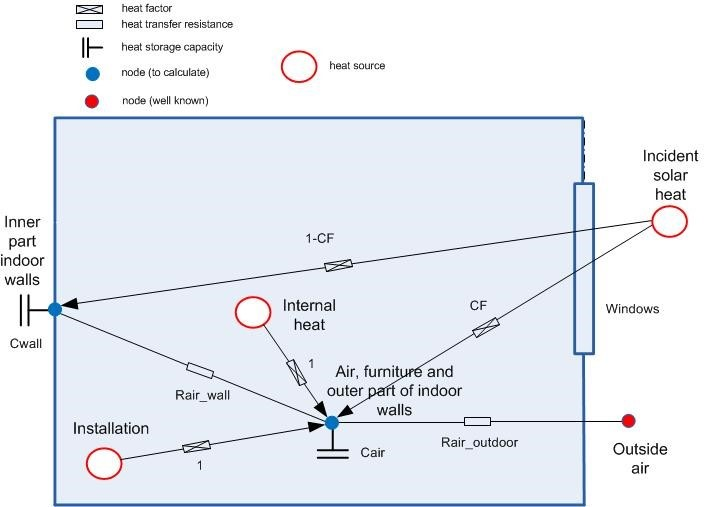
\includegraphics[width=1.0\columnwidth]{Pictures/envelopRC.jpg}
	\caption[Short title]{Schematic of envelope model}
	\label{fig:envelope2R2C}
	\end{figure} 
	
The equivalent electrical 2R-2C network with components and topology is given in Fig. \ref{fig:elec2R2C}.

\begin{figure}[H]
	\centering
	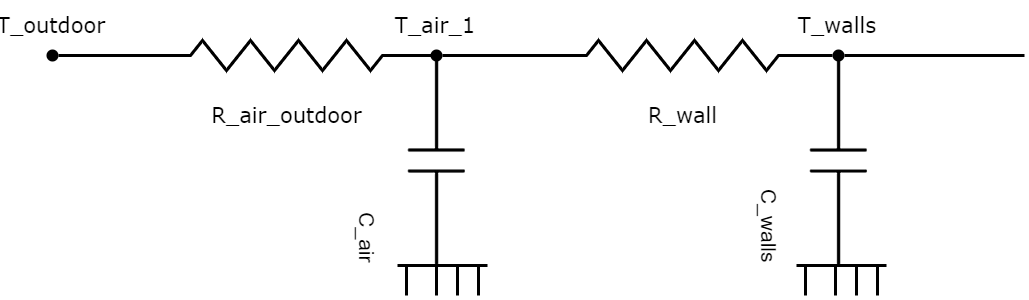
\includegraphics[width=1.0\columnwidth]{Pictures/2R2C_Model.png}
	\caption[Short title]{2R-2C house model}
	\label{fig:elec2R2C}
	\end{figure}
	
The model consists of two capacitances C\textsubscript{air, indoor} and C\textsubscript{wall} and two resistances R\textsubscript{wall} and R\textsubscript{air, outdoor}. The incident solar energy is divided between C\textsubscript{wall} and C\textsubscript{air} through the convection factor CF. It is assumed that both internal heat (lighting, occupancy and electric devices) and supplied heat (installation) initially heat up the indoor air. In Fig. \ref{fig:elec2R2C}, they are fully released at the T\textsubscript{air} node. 

 It is also assumed that furniture and the surface part of the walls have the same temperature as the air and the wall mass is divided between the air and wall mass. Thus, the capacity of the air node consists of the air capacity, furniture capacity and capacity of a part of the walls. \textbf{Appendix A} presents the coefficients in the dwelling model. In the resistance R\textsubscript{air, outdoor} the influence of heat transmission through the outdoor walls and natural ventilation is considered. 
 
For the air and wall nodes the following energy balances can be set up: 

\begin{equation}
C_{air}\frac{dT_{air}}{dt}=\frac{T_{outdoor}-T_{air}}{R_{air_{\_}outdoor}} + \frac{T_{wall}-T_{air}}{R_{air_{\_}wall}} + \dot{Q}_{inst} + \dot{Q}_{internal} + CF\cdot\dot{Q}_{solar}
\end{equation}

\begin{equation}
C_{wall}\frac{dT_{wall}}{dt}=\frac{T_{air}-T_{wall}}{R_{air_{\_}wall}} + (1-CF)\cdot\dot{Q}_{solar}
\end{equation}

 \begin{itemize}
      \item CF: Convection factor (solar radiation): the convection factor is the part of the solar radiation that enters the room and is released directly convectively into the room
      \item $\dot{Q}_{inst}$: delivered heat from heating system (radiator) [W].
      \item $\dot{Q}_{solar}$: heat from solar irradiation [W].
      \item $T_{air}$: indoor air temperature $^o$C.
      \item $T_{outdoor}$: outdoor temperature $^o$C.
      \item $T_{wall}$: wall temperature $^o$C.
      \item $R_{air_{\_}wall}$: walls surface resistance [$\frac{K}{W}$].
      \item $R_{air_{\_}outdoor}$: outdoor surface resistance [$\frac{K}{W}$].
      \item $C_{air}$: air capacity [$\frac{J}{K}$].
      \item $C_{wall}$: wall capacity [$\frac{J}{K}$].
    \end{itemize}
    

Total heat transfer of solar irradiation through the glass windows. 
\begin{equation}
Q_{solar}=g.\sum(A_{glass}.q_{solar})
\end{equation}

\begin{itemize}
    \item $q_{solar}$: solar radiation on the outdoor walls [$\frac{W}{m^2}$]. 
    \item g: g value of the glass (ZTA in dutch) [0..1]\cite{zontoetreding}
    \item A: glass surface [$m^2$].
\end{itemize}

%7.6.6.1.2 Ramen met niet-verstrooiende beglazing NTA8800
%https://help.dgmr.nl/bink9/zontoetredingsfactor-zta.html
%https://www.joostdevree.nl/shtmls/zta.shtml
%ISSO-Handboek Zonnestraling: 5.5.1 en 5.2

\newpage

\chapter{2 Zones house model 7R4C network}

The 4R-7C house model structure is implemented as described below:
	
\begin{figure}[H]
	\centering
	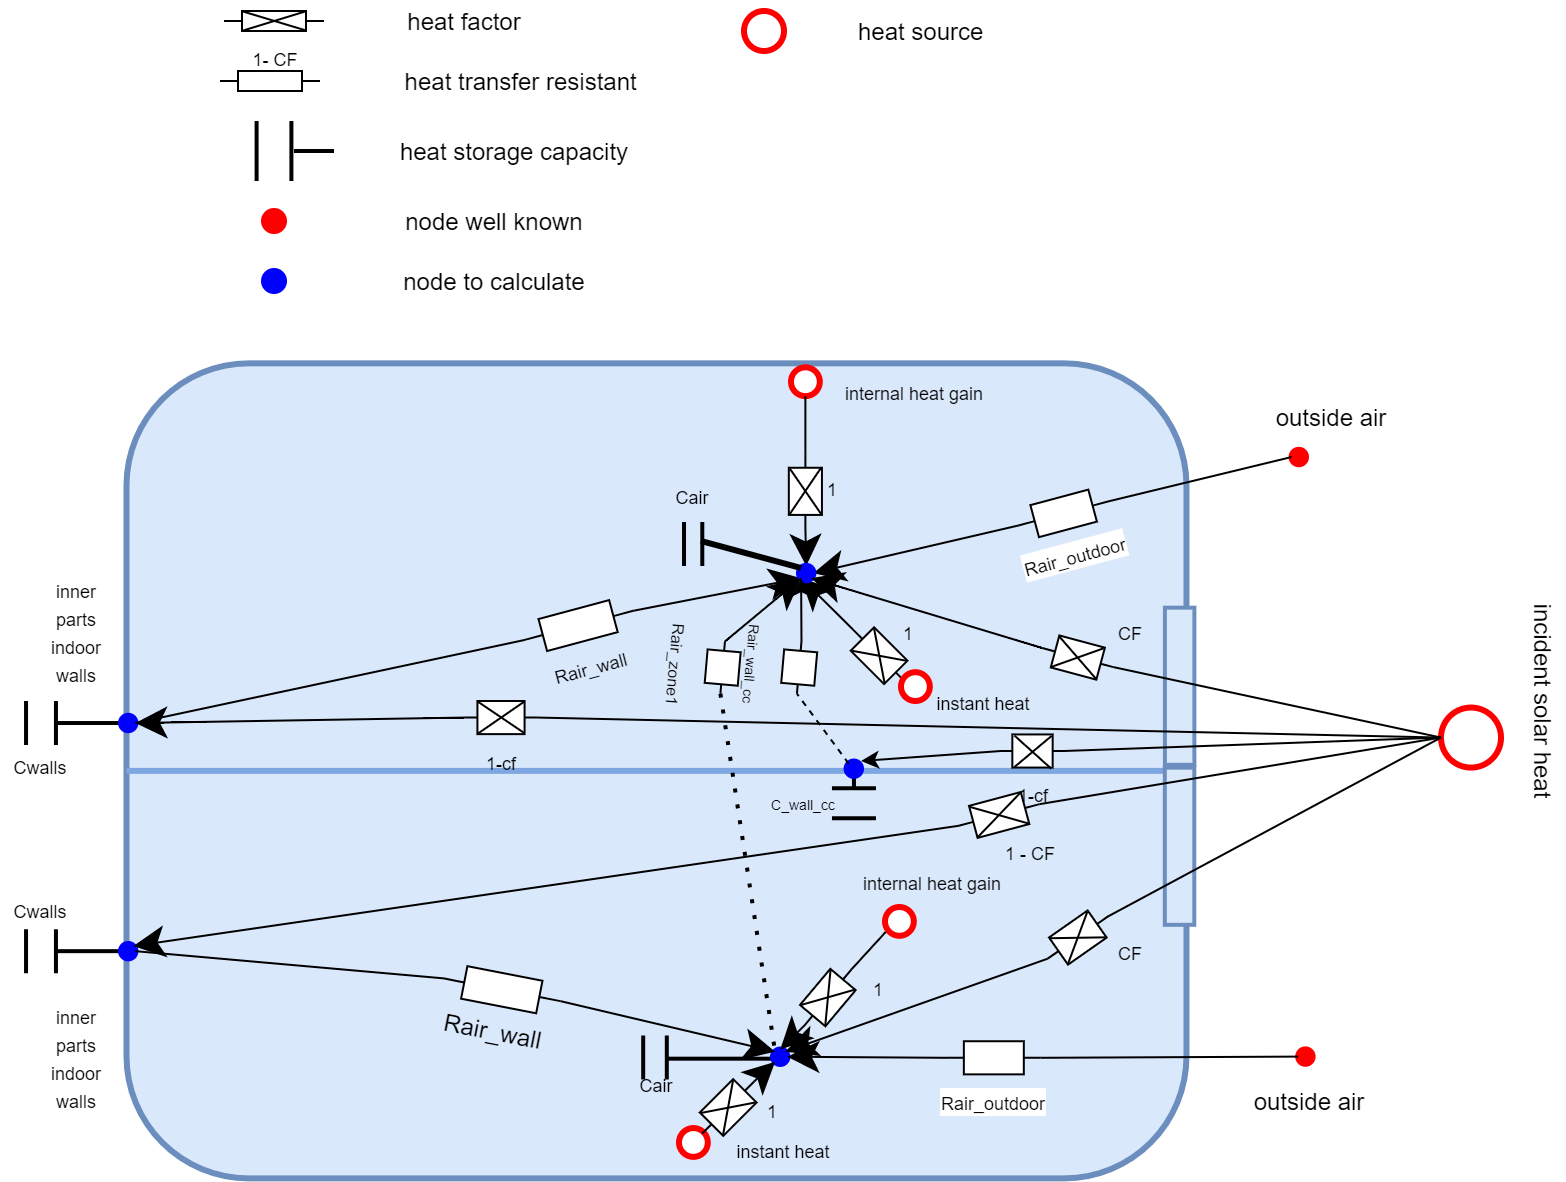
\includegraphics[width=1.0\columnwidth]{Pictures/House_electrical_circuits overview.png}
	\caption[Short title]{Schematic of a 2 zones house model}
	\label{fig:schema7R4C}
	\end{figure} 
	
The equivalent electrical 7R-4C network with components and topology is given in Fig. \ref{fig:elec7R4C}.

\begin{figure}[H]
	\centering
	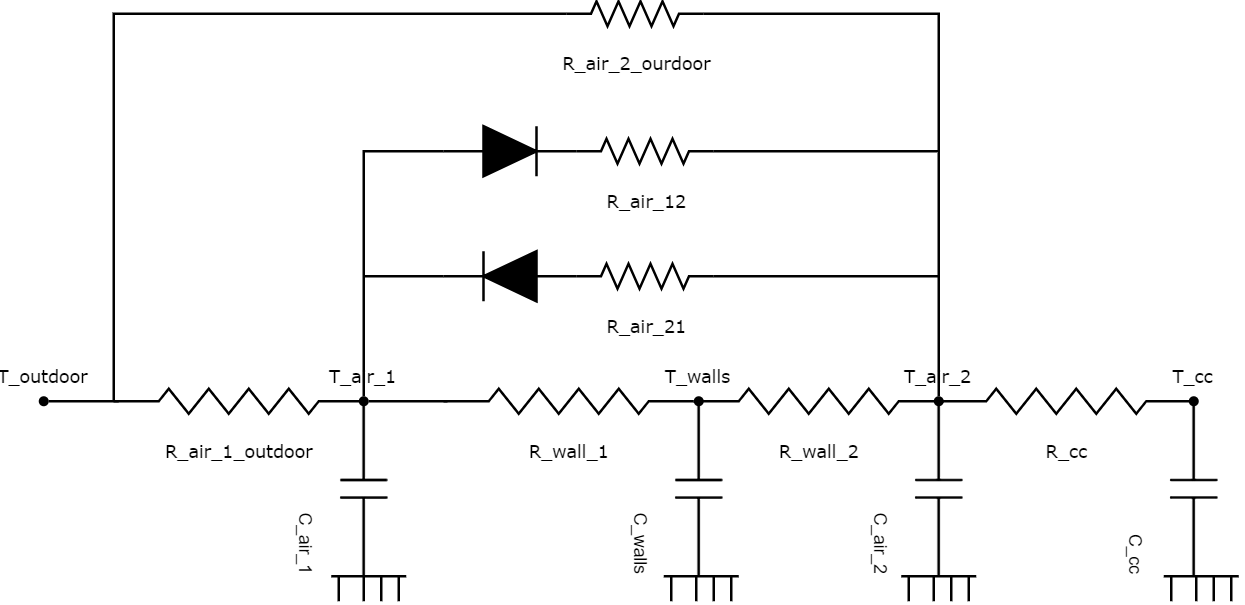
\includegraphics[width=1.0\columnwidth]{Pictures/2_Zones_house_circuits.png}
	\caption[Short title]{R-C circuits of 2 zones house model}
	\label{fig:elec7R4C}
	\end{figure}

with:\\
\begin{itemize}
    \item \texttt{T\_outdoor} : outdoor temperature [$\degr C$] 
    \item \texttt{T\_air\_1}  : zone 1 air temperature [$\degr C$]
    \item \texttt{T\_walls}   : wall temperature [$\degr C$]
    \item \texttt{T\_air\_2}  : zone 2 air temperature [$\degr C$]
    \item \texttt{T\_cc}      : temperature of the concrete layer between zone 1 and zone 2 [$\degr C$]
    \item \texttt{R\_air\_1\_outdoor} : outdoor resistance valus.
    \item \texttt{R\_wall\_1} : walls resistance value.
    \item \texttt{R\_wall\_2} : walls resistance value.
    \item \texttt{R\_cc}      : concrete resistance value.
    \item \texttt{R\_air\_12} : resistance value of air flow from zone 1 to zone 2.
    \item \texttt{R\_air\_21} : resistance value of air flow from zone 2 to zone 1.

\end{itemize}
\newpage

\section{NEN and ISO}

The list of NEN and ISO standard used in the calculation:

\begin{itemize}
    \item NTA 8800
    \item NEN 1068
    \item ISO 6946
    \item ISO 10077-2
    \item NEN 7120
\end{itemize}

\newpage


\bibliography{mybibliography}

\end{document}



